\chapter{Design} % (fold)
\label{cha:design}

\section{Software Architecture} % (fold)
\label{sec:software_architecture}
\subsection{Relationship with Cocoa Touch Framework} % (fold)
\label{sub:relationship_with_cocoa}

Core Data, Core Location, WebKit, MapKit, UIKit are used in this projects. As shown in Figure~\ref{fig:relationships},  NSManagedObject, NSObject, UITableViewController, UIViewController are inherited by different class in the project.
\label{sec:data_model}
\begin{figure}
	\centering
    \SetFigLayout{1}{1}
    {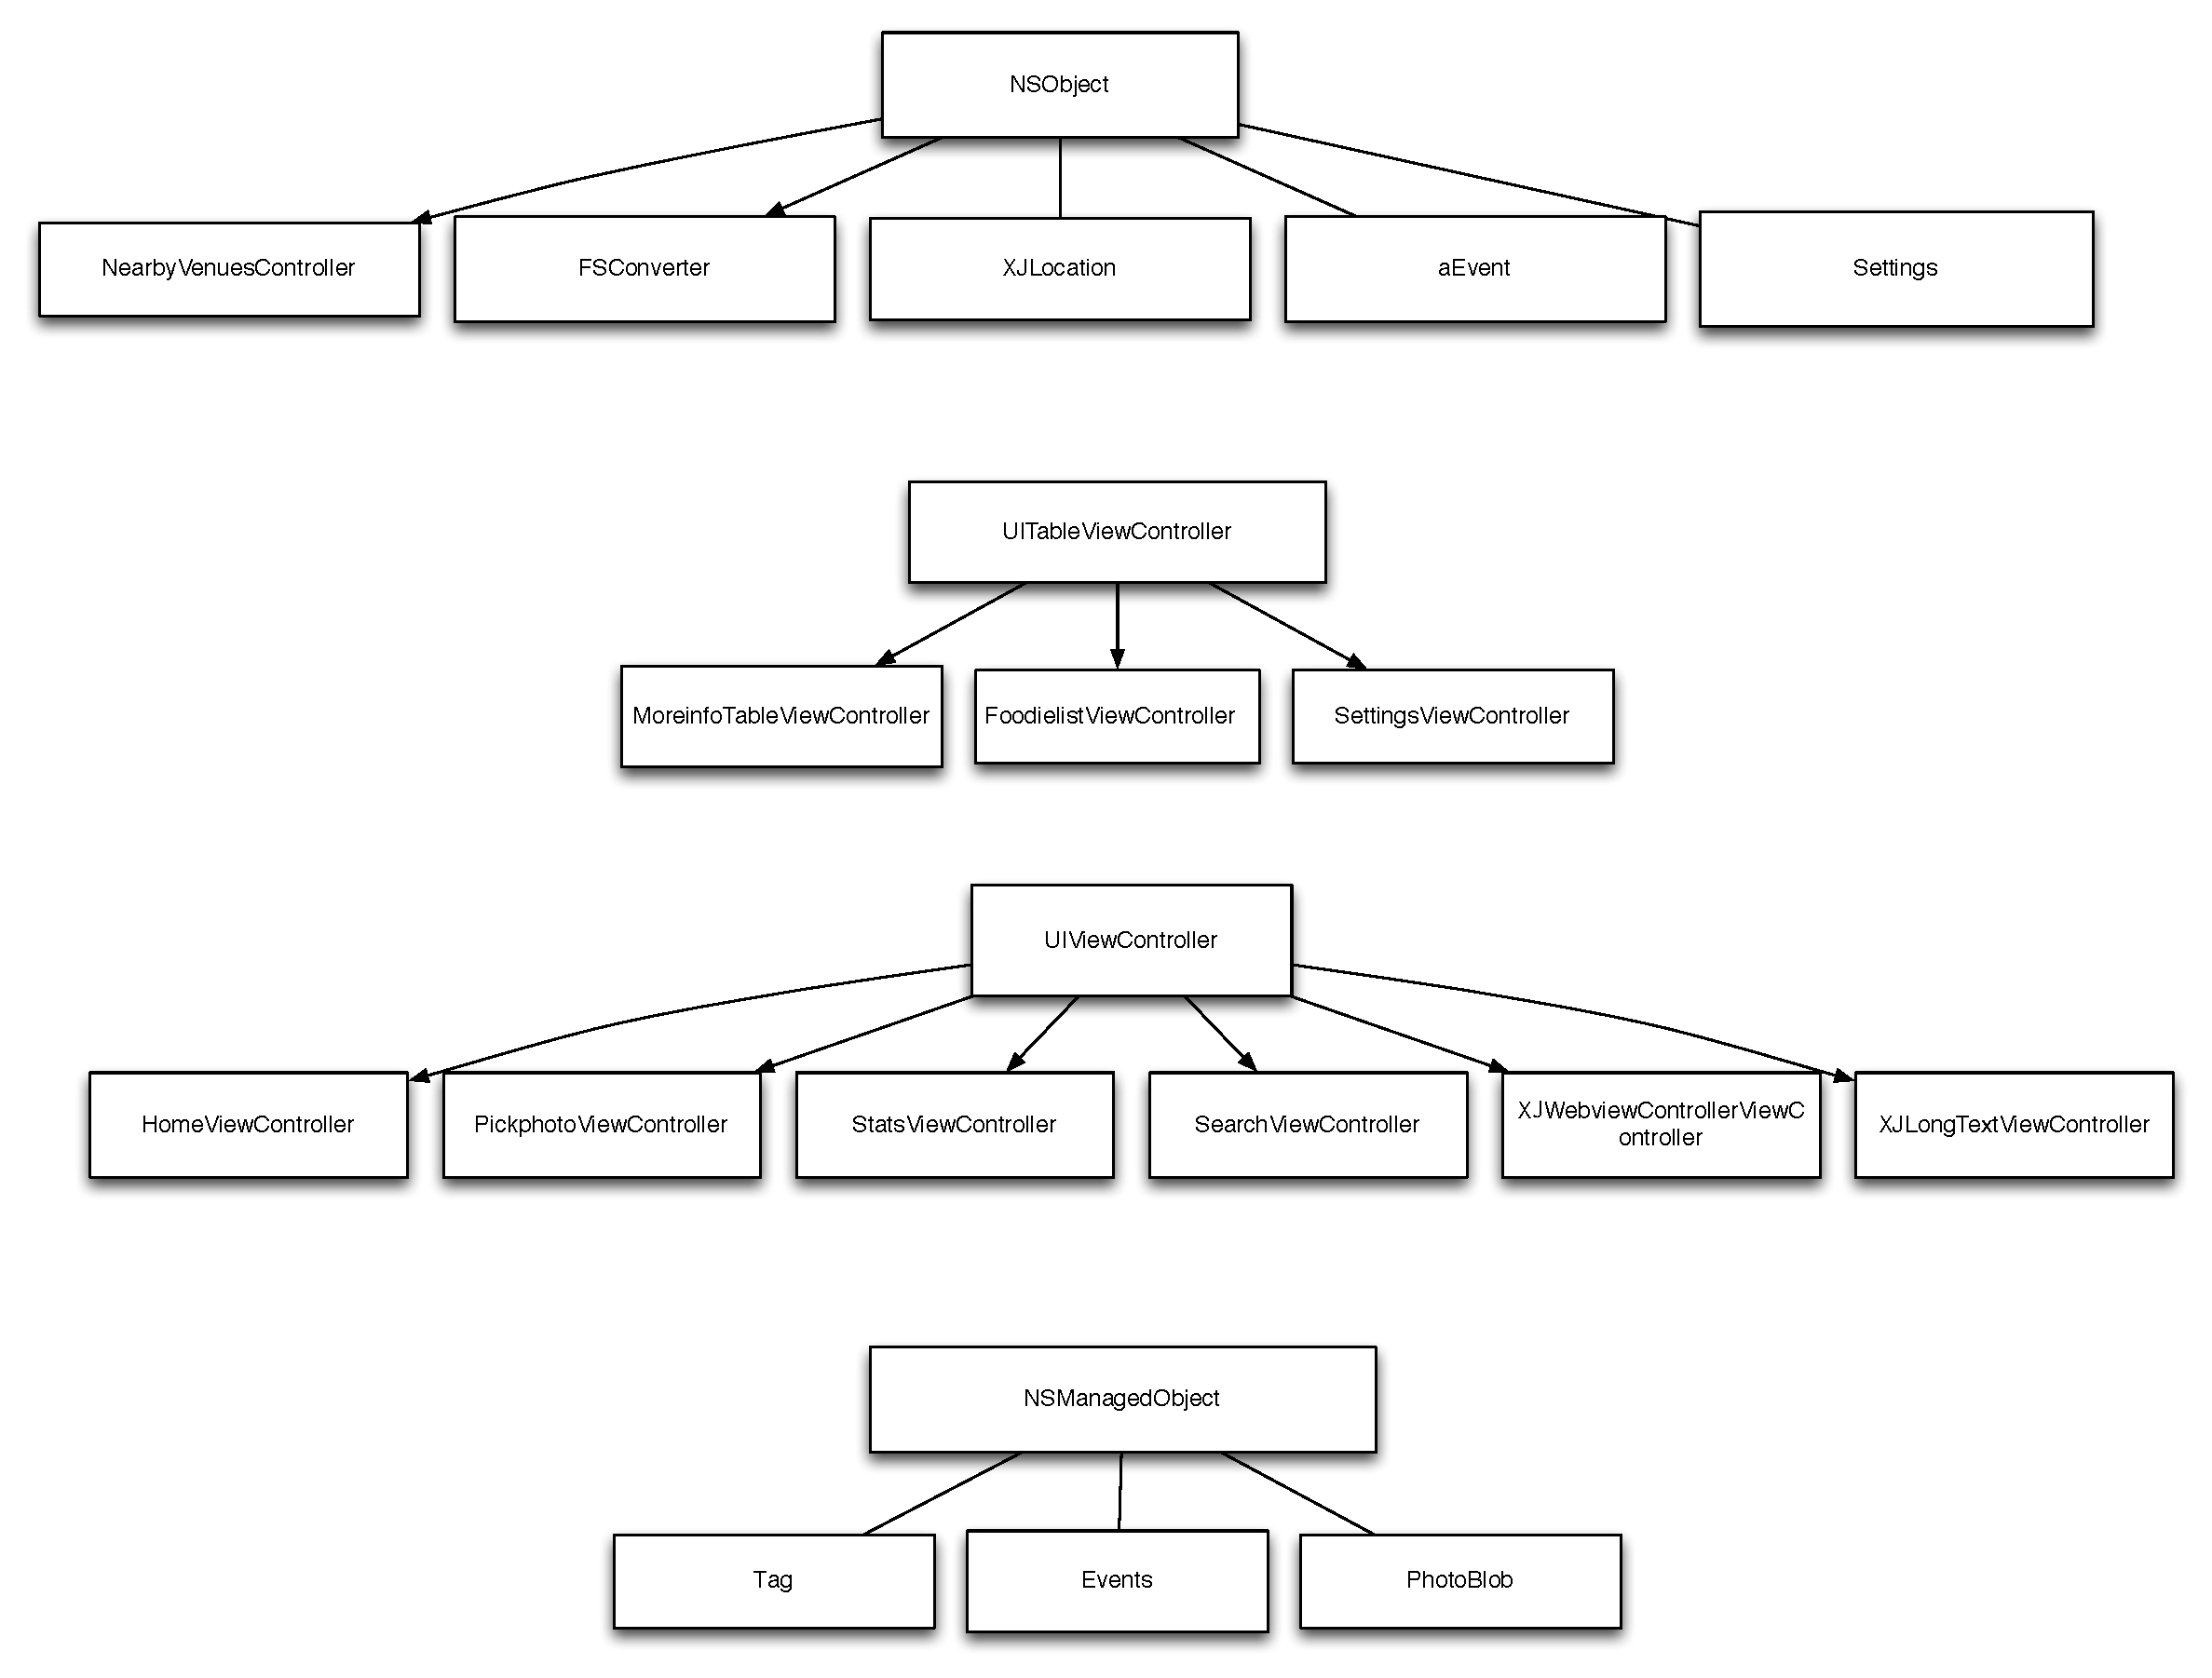
\includegraphics[%
    width=\figwidth, totalheight=\figheight, keepaspectratio]{./relationships.pdf}}
    \caption{Relationships with Cocoa Touch Framework}
	\label{fig:relationships}
\end{figure}
% subsection relationship_with_cocoa (end)
\subsection{Database Schema} % (fold)
\label{sub:database_schema}

	In this project, we used three table for storing all the information from users. As Figure~\ref{fig:data-schema} shows, Events is the main table in the app. It provides fields ``address'', ``comment'', ``creationDate'', ``latitude'', ``longitude'', ``locationName'', ``rate'', ``thumbnail'', ``photoBlob'' and ``tags''. ``address'' field is used when user didn't find their ``locationName'' in location List fetching from Foursquare API v2. ``Latitude'' and ``longitude'' is used for adding annotations in Map View. A 80*80 resolution thumbnail is stored for each event in order to accelerate loading in food list table. \\ 
	
	``photoBlob'' has one to one relationship with ``photo'' in PhotoBlob table. Using a separate table should also help speeding up when we don't need to load photo while we still need to get the meta data of the event. \\
	
	Field ``tags'' has many to many relationship with ``photos'' in Tag table since one photo can labeled with many tags and one tag can relate to many photos.  
	

\begin{figure}
	\centering
    \SetFigLayout{1}{1}
    {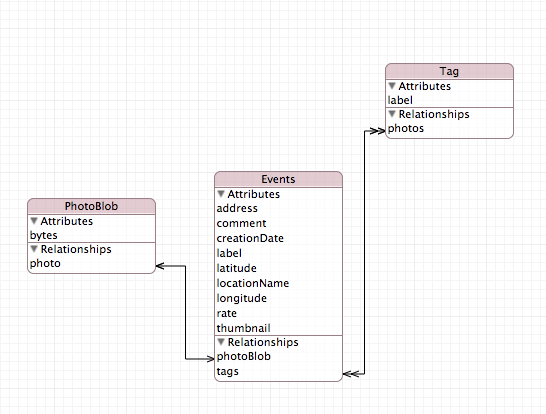
\includegraphics[%
    width=\figwidth, totalheight=\figheight, keepaspectratio]{./screenshots/database_schema.png}}
    \caption{Database Schema}
	\label{fig:data-schema}
\end{figure}

% subsection database_schema (end)

\subsection{Settings Property List} % (fold)
\label{sub:settings_list}

	When developing iOS, we can also use another way to store data we need. Property List is used to store all information related to the app itself. For instance, using Property List to store App Display Name, App Version are commonly used in all apps for iPhone. \\
	
	``Fancy Foodie'' uses release number as main version string and git hash tag of the release as build string, so ``1.0 (build 98a9e84)'' is shown in Figure~\ref{fig:settings} which means that the main version number is 1.0 and build hash tag is 98a9e84. \\
	 
	 This app also use property list to store whether we need to save photo to album locally. If this option is enabled, the app will create a album  named ``Fancy Foodie Photos'' and put photos in this album as shown in Figure~\ref{fig:album}.
% subsection settings_list (end)
% section software_architecture (end)



\section{Modules} % (fold)
\label{sec:modules}


\begin{figure}
	\centering
    \SetFigLayout{1}{1}
    {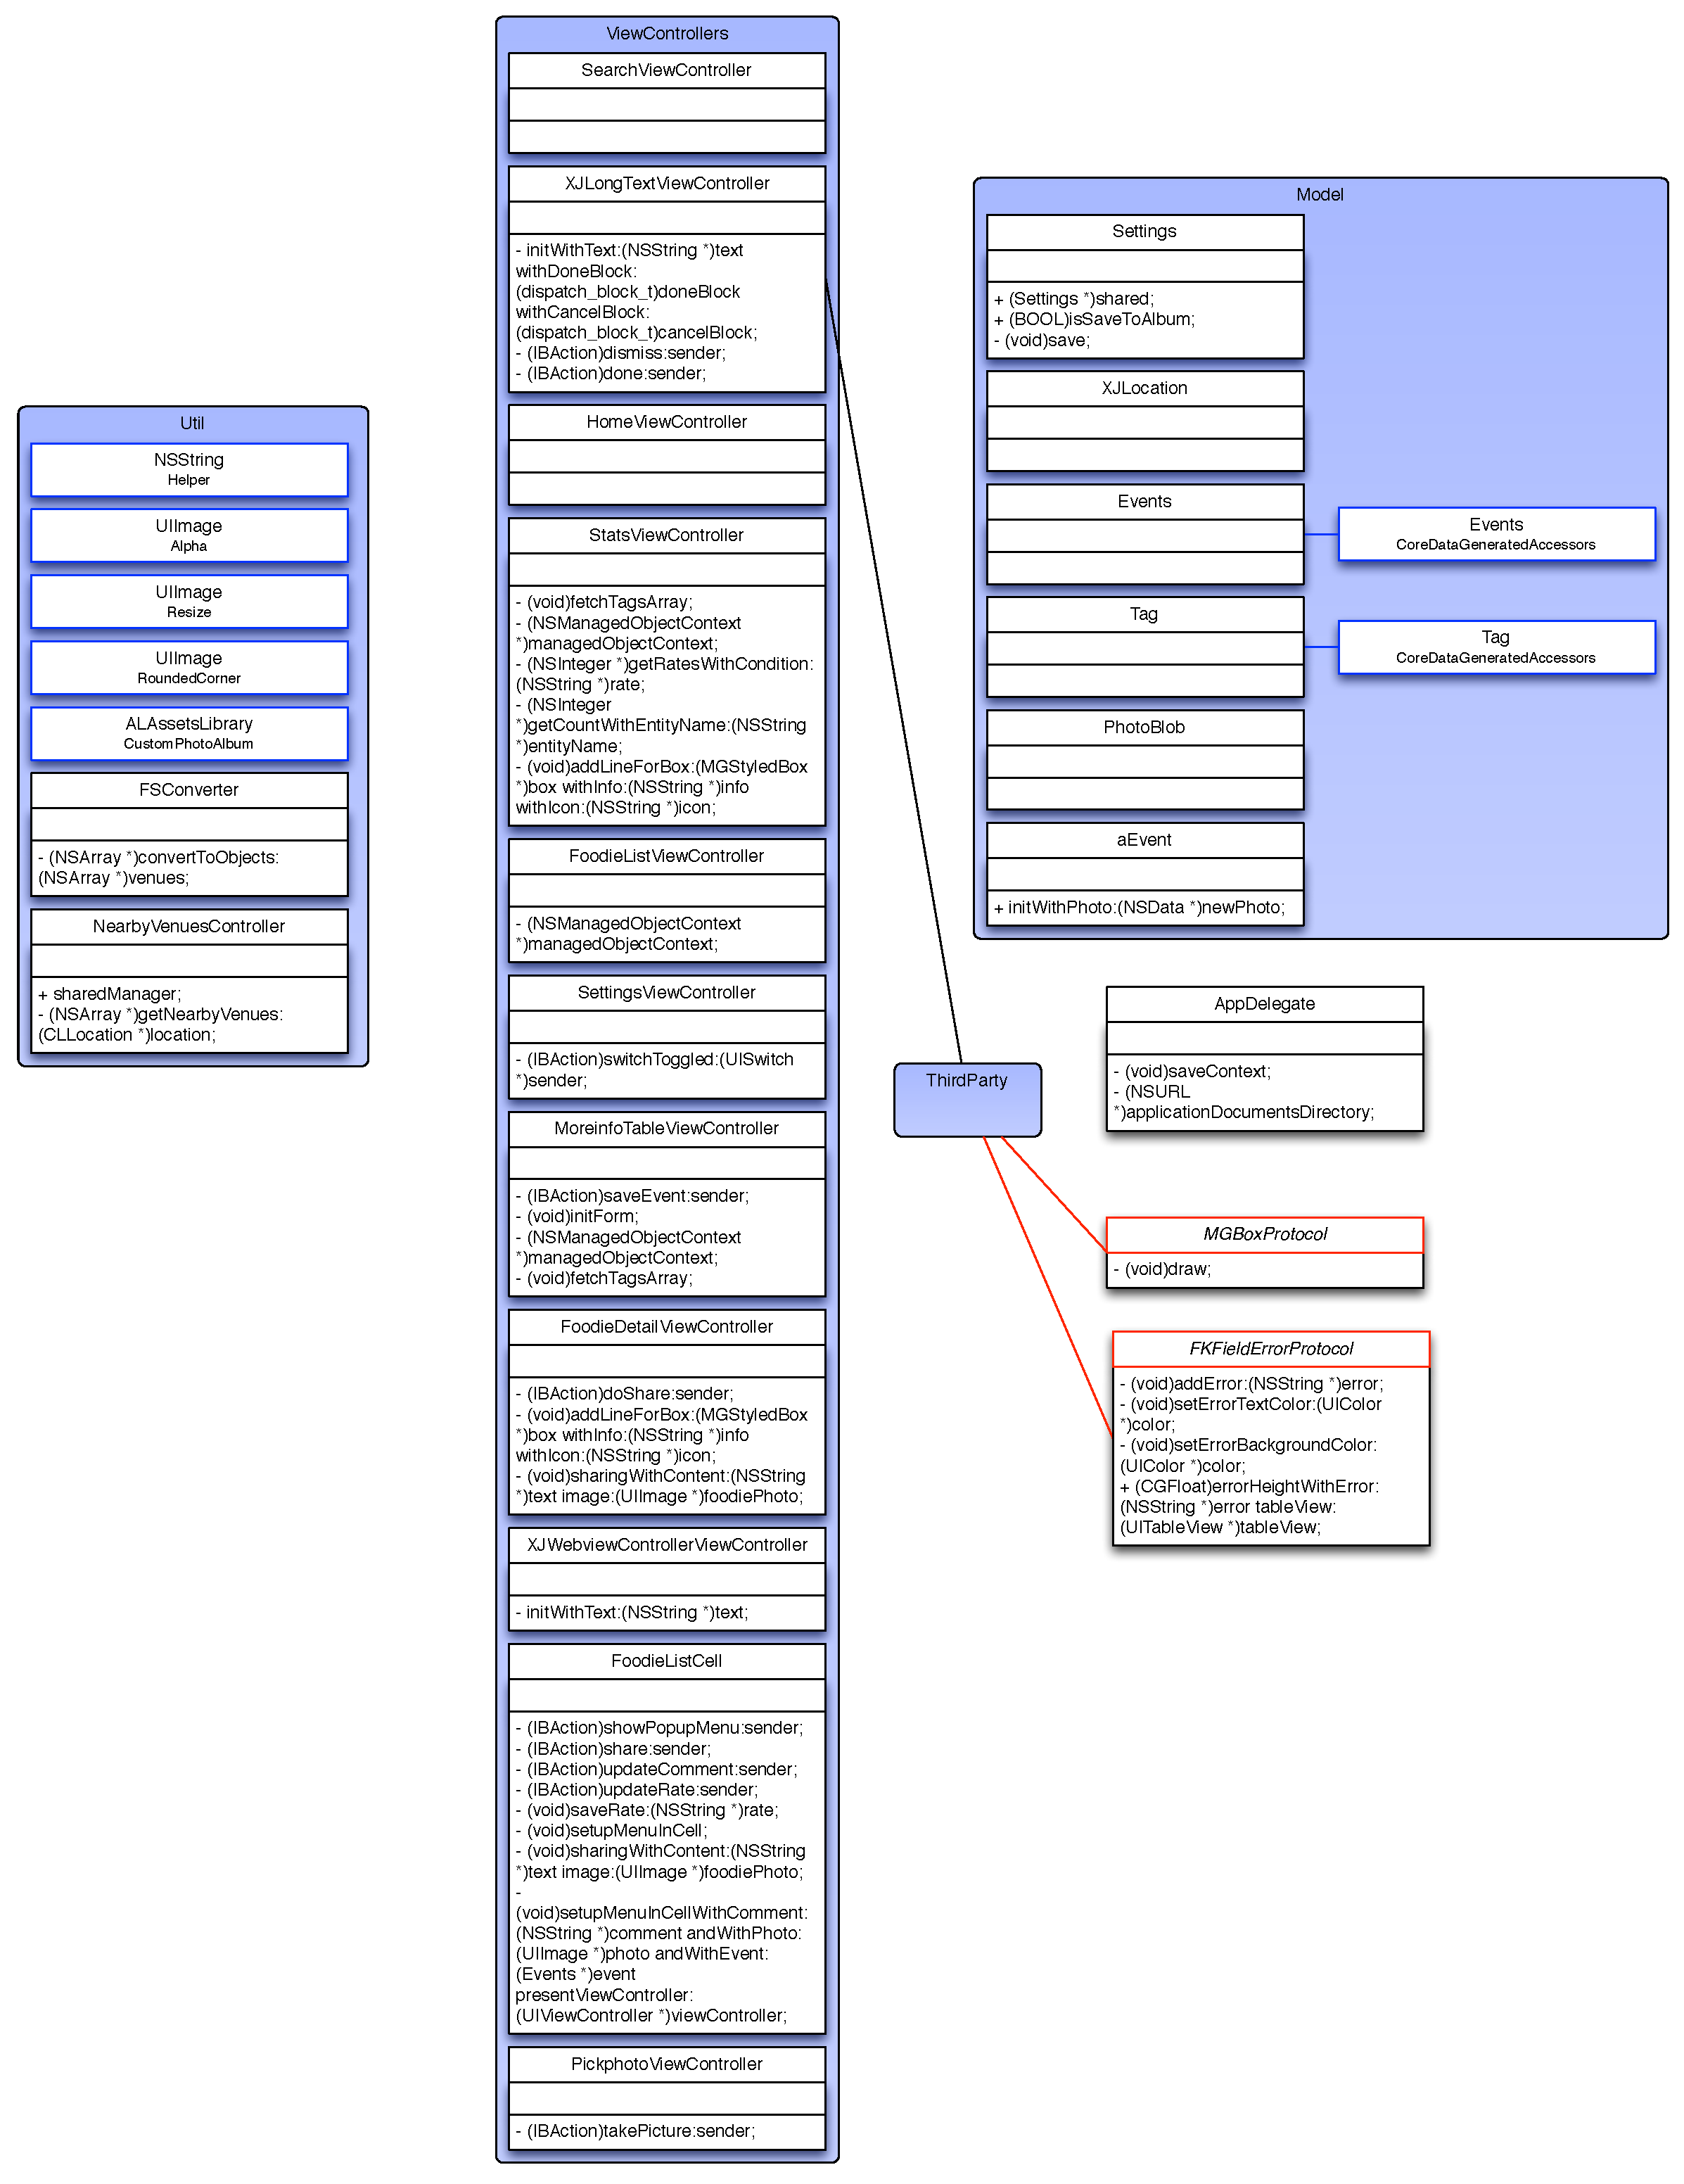
\includegraphics[%
    width=\figwidth, totalheight=\figheight, keepaspectratio]{./UML_Fancy.pdf}}
    \caption{Class-diagram of the project}
	\label{fig:classdiagram}
\end{figure}
% subsection overview_of_modules (end)

\subsection{View Controllers} % (fold)
\label{sub:view_controllers}

% subsection view_controllers (end)
 	 
\subsection{Data Models} % (fold)
\label{sub:models}

% subsection models (end)

\subsection{Third party libraries and Utilities} % (fold)
\label{sub:third_party_and_utilities}
The following is a list of third party libraries used in the project.
		\begin{itemize}
		    \item TestFightSDK: Beta Testing on the fly.
		    \item BaseKit: Tools to create singleton class and better Location Manager.
			\item QBPopupMenu: Popup Menu User Interface
			\item CZPhotoPickerController: Preview of photos and better photo picker.
			\item FormKit: Form style tableview creation.
			\item BButton: Button with twitter bootstrap color schema.
			\item Foursquare2: Foursquare API version 2.
			\item MGBox: Table style boxes creation.
			\item SORelativeDateTranformer: Convert date to relative date such as ``One day ago''.
			\item FontAwesome: Adding icons to user interface.
			\item SVProgressHUD: Notification messages display.
		 \end{itemize}

% subsection third_party_and_utilities (end)
% section modules (end)

\section{Key Methods} % (fold)
\label{sec:main_methods}

\subsection{Insert New Event} % (fold)
\label{sub:insert_new_event}
	Figure~\ref{fig:storyboard-home} shows the 
% subsection insert_new_event (end)

\subsection{Update Event} % (fold)
\label{sub:update_event}


% subsection update_event (end)

\subsection{Delete Event} % (fold)
\label{sub:delete_event}

	Delete event is very simple in this app. In food list tab, you'll see a list of 
% subsection delete_event (end)

\subsection{Searching Events} % (fold)
\label{sub:searching_logic}
	
	Searching events is done with MapKit API. All the events are fetched in during loading time. The events are annotated with red pins when the tab is loaded.   \\
	As shown in Figure~\ref{fig:map-address}, as the user is typing in the address, the searching string is passed to search controller, so at the same time, we're using geo coder to guess the possible locations for that string. The possible locations are displayed in a table view. After the use choose one possible location, the central region will be focused on that area. At this time, the nearby events stored in database will appear in front of the user.
	

% section main_methods (end)
% chapter design (end)